\documentclass{article}
\usepackage{graphicx}
\usepackage{multicol} % use to multiple column in itemize
\usepackage{float}
\usepackage{setspace}
\usepackage{hyperref}
\setlength{\parskip}{0.5em}

\begin{document}

\title{Reinforcement Learning}
% \author{Cong Cuong PHAM}

\maketitle

\begin{abstract}
This document introduces some fundamental notions of Reinforcement Learning.
\end{abstract}

\subsection{Reinforcement Learning}
\par The goal of reinforcement learning is to maximize a cumulative reward function (or equivalently, minimize a cumulative cost function), given a set of actions and results. Reinforcement learning is modeled to mimic the way we learn in the real world. We try to solve problems using different techniques. Most of the time, nothing of merit results from our experiments. But occasionally, we stumble upon a set of actions that result in a sweet reward. When this happens, we attempt to repeat these actions that will result in our getting rewarded. If we are rewarded yet again, we further associate those actions with the reward and that is known as the reinforcement cycle. The entire process is also known as performance maximization.

\begin{figure}[H]
\centering
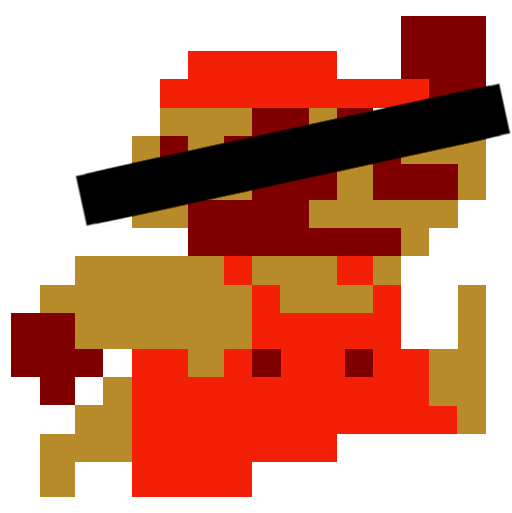
\includegraphics[width=0.6\linewidth]{pic/reinforcement-learning.png}
\caption{Example of reinforcement learning.}
\end{figure}

More examples

\begin{itemize}
    \item Discover how to fly a quadcopter by minimizing the function which evaluates the chances of crashing.
    \item Learn to beat a video game like 'Super Mario Bros.' by minimizing the time it takes to get to the castle.
    \item Attempt to take a photo and ``re-draw'' it in the style of a particular artist.
    \item Automate the trading of stocks and securities by maximizing profit and minimizing transaction fees.
\end{itemize}

\par Reinforcement learning is actually a completely different category of learning from supervised and unsupervised learning. It's closer to supervised learning than it is to unsupervised learning, but you could get away with calling it semi-supervised learning. To learn more about reinforcement learning, take a look at the dive deeper section. We won't return to reinforcement learning in this class, but it's important to be aware of it as a data scientist. Much work has been done using reinforcement learning and deep neural networks that are of benefit to machine learning.
\begin{flushright}
    source: \href{https://courses.edx.org/courses/course-v1:Microsoft+DAT210x+6T2016/courseware/e36e6b45ae5d4032bef2ec557c1ff48f/a8cf8333f6044e9b9a357b7797f282e3/?child=first}{course.edx.org}  
\end{flushright}
\end{document}